\section{Experimental Setup}\label{s:5}

We use SUMO for microscopic traffic simulation, with SUMO-RL providing the
Gymnasium interface for the RL agents. TraCI retrieves traffic states and
updates signal phases. The simulations run headlessly, while network, timing,
scenario, reward, and learning parameters are specified in YAML configuration
files. The simulated road network models the Ly Thai To intersection in Ho
Chi Minh City, as illustrated in Fig.~\ref{fig:road-network}.

\begin{figure}[htbp]
\centering
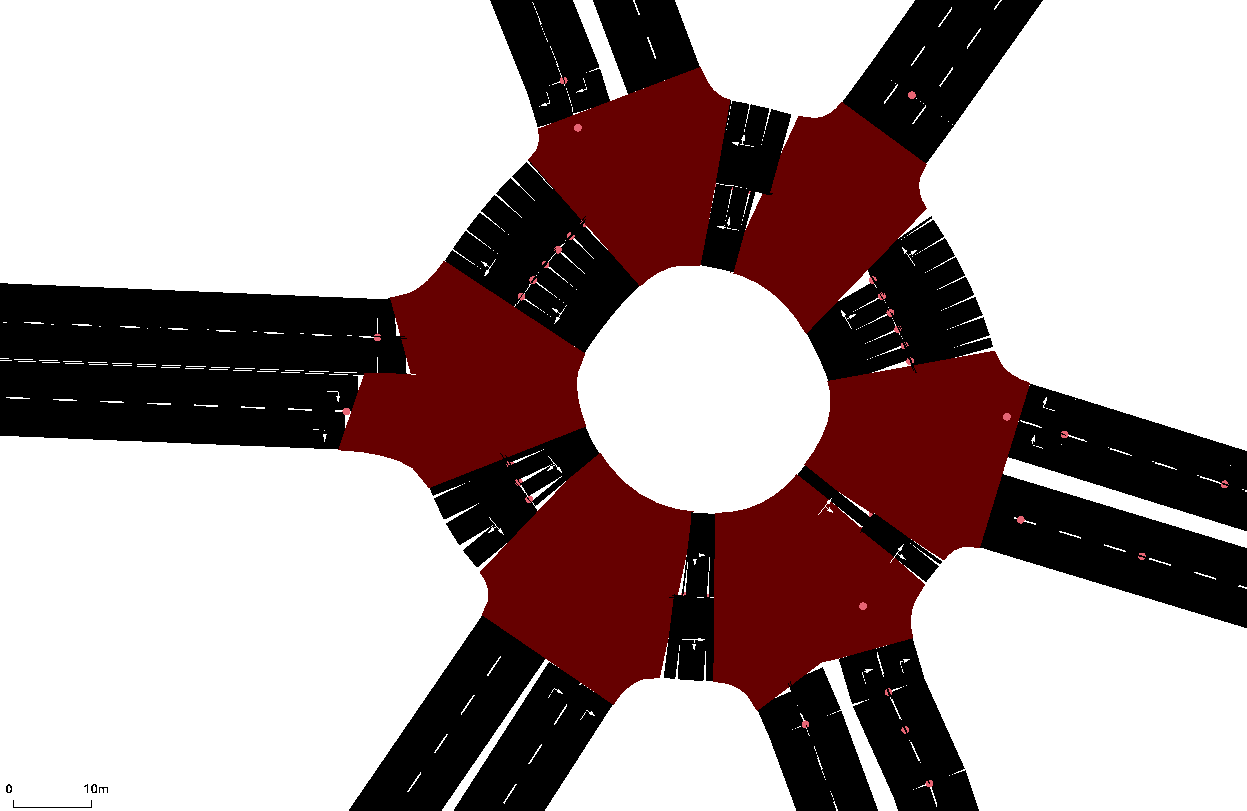
\includegraphics[width=\columnwidth]{figures/road_network.png}
\caption{SUMO road-network model based on the Ly Thai To seven-way intersection.}
\label{fig:road-network}
\end{figure}

% TODO: Replace [X] with the exact software versions used in the final runs.
The experiments use SUMO [X] and SUMO-RL [X]. Additional software versions are
Gymnasium [X], Stable-Baselines3 [X], and PyTorch [X].

\subsection{Network and Traffic Demand}

% TODO: Confirm whether the modeled intersection is described as a
% six-approach roundabout or a seven-way intersection in the final paper.
The controlled road network is based on the Ly Thai To intersection and is
represented by a seven-way road layout. The network model is stored in the
official roundabout network file. It contains [N-in] inbound
approaches, [N-out] outbound approaches, and [L] circulatory lanes. The central
traffic signal is \texttt{[signal ID]}, and the controlled program is
\texttt{[program ID]}.

% TODO: Verify the exact approach labels and lane counts from the final network.
The main inbound approaches are [TODO: list approach IDs, e.g. A1--A4 and A6].
Each inbound approach has [TODO: number of lanes per approach or a lane table].
The system also includes [TODO: number] circulatory segments, identified in the
simulation as [TODO: list segment IDs].

The simulated traffic consists of mixed vehicle classes, including passenger
cars, buses, trucks, motorcycles, and emergency vehicles. Vehicle-type
definitions are provided in
\texttt{[TODO: Add sth]}. The vehicle proportions
and vehicle definitions used in the final experiments are summarized in
Table~\ref{tab:traffic_demand}.

% TODO: Replace the demand values with the final scenario values.
% Confirm whether values are vehicles/hour, vehicles/episode, or both.
\begin{table}[t]
\caption{Traffic-demand scenarios and vehicle mixes.}
\label{tab:traffic_demand}
\centering
\small
\begin{tabular}{lccccc}
\hline
\textbf{Scenario} & \textbf{A1} & \textbf{A2} & \textbf{A3}
& \textbf{A4} & \textbf{A6} \\
\hline
Morning peak      & 4200 & 1800 & 2600 & 2100 & 2400 \\
Evening rush      & 2200 & 4200 & 2100 & 3100 & 3200 \\
Midday balanced   & 2400 & 2200 & 1900 & 1800 & 2000 \\
School commute    & 2800 & 2500 & 3200 & 2400 & 2500 \\
Late-night flow   & 650 & 600 & 450 & 400 & 550 \\
\texttt{[X]} & \texttt{[X]} & \texttt{[X]} & \texttt{[X]} & \texttt{[X]} & \texttt{[X]} \\
\hline
\end{tabular}
\begin{minipage}{\columnwidth}
\footnotesize
\textit{Demand unit: [TODO: vehicles/hour or vehicles/episode].}\par
\textit{Vehicle proportions: [TODO: link each scenario to its route file
and provide the final vehicle mix.]}
\end{minipage}
\end{table}

The route scenarios are selected from the project scenario manifest. The
training scenarios belong to the \texttt{TR} split, the validation scenarios
belong to the \texttt{VA} split, and the test scenarios belong to the
\texttt{TE} split. The complete list of route files used in the final
experiments is reported in Table~\ref{tab:scenario_splits}.

% TODO: Add the actual route filenames and scenario IDs.
\begin{table}[t]
\caption{Scenario allocation for training, validation, and testing.}
\label{tab:scenario_splits}
\centering
\begin{tabular}{lll}
\hline
\textbf{Split} & \textbf{Scenario ID(s)} & \textbf{Route file(s)} \\
\hline
Training     & [TODO] & [TODO] \\
Validation   & [TODO] & [TODO] \\
Test         & [TODO] & [TODO] \\
\hline
\end{tabular}
\end{table}

For each episode, the environment loads one route file and terminates after
[TODO: 3600] seconds or the episode's configured termination condition.
The number of training scenarios, validation scenarios, test scenarios, and
episodes per scenario will be reported after all experiments are completed.